\documentclass[11pt]{article}            % Report class in 11 points
\parindent0pt  \parskip10pt             % make block paragraphs
\usepackage{graphicx}
\usepackage{listings}
\graphicspath{ {images/} }
\usepackage{graphicx} %  graphics header file
\begin{document}
\begin{titlepage}
    \centering
  \vfill
    
\includegraphics[width=8cm]{uni_logo.png} \\ 
	\vskip2cm
    {\bfseries\Large
	Artificial Intelligence \\ (CS13217)\\
	
	\vskip2cm
	Lab Report 
	 
	\vskip2cm
	}    

\begin{center}
\begin{tabular}{ l l  } 

Name: & Anam bibi\\ 
Registration \#: & CSU-S15-118 \\ 
Lab Report \#: & 03 \\ 
 Dated:& 30-03-2018\\ 
Submitted To:& Mr. Usman Ahmed\\ 

 %\hline
\end{tabular}
\end{center}
    \vfill
    The University of Lahore, Islamabad Campus\\
Department of Computer Science \& Information Technology
\end{titlepage}


    
    {\bfseries\Large
\centering
	Experiment \# 3 \\

Implementing Deapth First Search\\
	
	}    
 \vskip1cm
 \textbf {Objective}\\  To understand and implement the deapth first search.
 
 \textbf {Software Tool} \\
1.  operating system window 10\\
2.  sublime version 3.0 \\
3.  python\\
\section{Theory }              
 Depth-first search (DFS) is an algorithm for traversing or searching tree or graph data structures. One starts at the root (selecting some arbitrary node as the root in the case of a graph) and explores as far as possible along each branch before backtracking.\\
DFS, is a way to traverse the graph. Initially it allows visiting vertices of the graph only, but there are hundreds of algorithms for graphs, which are based on DFS. Therefore, understanding the principles of depth-first search is quite important to move ahead into the graph theory. The principle of the algorithm is quite simple: to go forward (in depth) while there is such possibility, otherwise to backtrack.\\	
This algorithm has following 5 steps: \\
1Select a source node. \\
2.Check the untraversed edges out of that node.\\
3.If found then traverse through one of the untraversed edge to its child vertex.\\
4.Check if child vertex have any untraversed edges out of it.\\
If yes, then repeat from Step 3.\\
Else return the element and backtrack to its parent node and repeat from Step 2.\\
5.If not then check if any undiscovered vertices remains.\\
If yes, then repeat from Step 1.\\
Else terminate the execution.\\
\section{Task}  
\subsection{Procedure: Task 1 }     

\begin{figure*}
\centering
  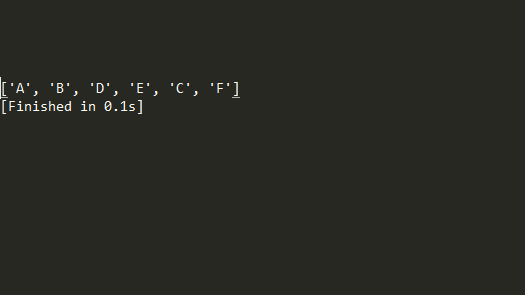
\includegraphics[width=12cm,height=6cm,keepaspectratio]{1.png}
\caption{Time Independent Feature Set}
\label{Figure:3}    
\end{figure*}

\begin{lstlisting}[language=Python]
graph1 = {
    'A' : ['B','C'],
    'B' : ['D','E'],
    'C' : ['A','E'],
    'D' : ['B','E'],
    'E' : ['C','F','D','B'],
    'F' : ['D','E'],
}

def dfs(graph, node, visited):
    if node not in visited:
        visited.append(node)
        for n in graph[node]:
            dfs(graph,n, visited)
    return visited

visited = dfs(graph1,'A', [])
print(visited)
\end{lstlisting}
\section{Conclusion}  
Depth first search is an interesting algorithm, and as you might suspect, it is particularly well suited for inspecting if a graph is connected; if the tree returned by depth first search contains all vertices in the graph, it is connected, otherwise, it is not.

 
\end{document}                          % The required last line
